\chapter{System}

This chapter contains the state-of-the-art of the system, the design of the application architecture, the design of the scanning methodology, and the description of the Agile method used to develop the application.

% •	Description of the application architecture suitable for security scanning (executable, terminal, later ui)
%%% o	System Settings UI and API to control every aspect of the device
% •	Agile method, stories, backlog

% IEC62443 findings and table
% Go language
% Explanation of the libraries used (Cobra for CLI, Zerolog for logging) and their benefits
% •	Design of the scanning methodology.
%%% o	Aspects covered: Outdated OS, outdated libraries (e.g., OpenSSL), outdated software, default or weak credentials, insecure network communication, …

\section{Companies}

The company where we did our internship is located in the province of Verona in Italy. It's owned by a holding group which controls some other companies and startups, all located in the same place. It includes the main company, which is the one that designs and produces the industrial devices, and another company.

The latter is the business where we are enrolled for the internship; it is in charge of the development of management software that allows these devices to become domotic, that is industrial automation, in order to send and receive data from the cloud, to be able to interact with the device remotely, and to be able to monitor the status of the device. The software is a built-in service running on the hardware, and all the data are collected and sent to the cloud through the company's servers.

Since the businesses are under the same holding group, they share administrative resources and also technical resources. From now on, we refer to the main (or first) company talking about standards, regulations and devices, and to the second one talking about the software and the cloud.

\subsection{Software company organization}

The cloud management software, developed by the second company, is composed of five main layers and it is managed by five different teams:
\begin{itemize}
  \item \textbf{Device}: it should make the adoption of the platform, and it handles the cloud lifecycle of a device, by managing the device registration and configuration of the service on the hardware and the server-side handling of the collected data to being able to create flexible dashboards and reports;
  \item \textbf{VPN}: it handles the connection to a device through a VPN, and it is in charge of the security of the connection;
  \item \textbf{Apps}: the work of the apps team is to increase the value of the platform, by allowing third parties to integrate their services with the platform, and by creating apps that can be installed on the devices. Customers can craft their own apps by using the provided \textit{Software Development Kit} (SDK), that is a set of tools and documentation;
  \item \textbf{Core}: it is the core of the platform, and it in responsible for the provided backend REST APIs mainly used for the frontend website. It also handles the management of the user via a custom \textit{IDentity Provider} (IDP);
  \item \textbf{Platform}: last but not least, the platform team orchestrate all the infrastructure needed to run the services, and it is in charge of the deployment of the services on the cloud. It is also responsible for the monitoring of the services, and for the security of the development lifecycle and deploy process.
\end{itemize}

The cloud software is developed using the microservices architecture, that is a design pattern that structures an application as a collection of loosely coupled services. Services can be developed, deployed, and scaled independently.

We were virtually part of the apps team, and we were in charge of developing a scanning tool that can be used to check the security of the devices and to report the issues to the user.

\section{Deployment of the microservices}

This section explains how a software can be deployed in a cloud environment, with a focus on the microservices architecture.

% microservices are docker container
% kubernetes
% helm
% CI/CD by testing
% terraform?

\subsection{Microservice}

Microservice architecture is an architectural style that structures an application as a collection of services that are independently deployable and loosely coupled. Independently deployable means that a service is packaged as a executable unit and is production-ready. Loosely coupled means that the different services are not directly dependent on each other, and they can be developed, deployed, and scaled independently.~\cite{microservices-what-are}

\subsection{Virtualization}

Virtualization is a technology that allows the creation of virtual representations of physical resources such as processors, storage devices or network devices. Virtual software mimics the functions of physical hardware, allowing multiple operating systems to run on a single physical machine. Virtualization can increase IT agility, flexibility, and scalability while creating significant cost savings due to the abstracting of the physical hardware.~\cite{virtualization-aws}

Each virtualized environment runs within its allocated resources. There are two main types of virtualization approaches: container-based virtualization and hypervisor-based virtualization, also known as virtual machines' virtualization.

\subsection{Container vs. Virtual Machine}

A modern and efficient way to execute microservices is to use \textit{containers}. \\
Containers are lightweight software packages that contain all the dependencies required to execute the contained software application in a virtualized environment. They share the same kernel of the host system, but they are usually isolated from the host and from other containers and they can run different operating systems. Another advantage of containers is that they are immutable, meaning that they could be altered after their creation, but the state is restored at each execution, without considering possible further different configurations.\\
Instead, compared to the containers, \textit{virtual machines}'s goal is to virtualize the entire system hardware, therefore they are slower and heavier - resources side and disk usage side - than containers.

The company uses \textit{Docker}\footnote{\url{https://www.docker.com}} to create, deploy, and run containers. Docker is an application that allows developers to build, package, and run applications as containers.

Docker itself enables the user to instantiate a single container at time from an image, that is a series of instructions that defines the environment of the container, starting from the base operating system up to all the steps needed to install the final software. Since we are talking of a microservices architecture, there is the need to run multiple containers at the same time, and to manage them, from the creation to the destruction up to the recovery in case of failure or the scaling in case of high load. This is where we need an orchestration tool.

\subsection{Orchestration}

The containers are managed by \textit{Kubernetes}\footnote{\url{https://kubernetes.io}}, also known as \textit{K8s}, an open-source container orchestration platform that automates the deployment, scaling, and management of containerized applications. Kubernetes provides a platform for automating the deployment, scaling, and operations of application containers across clusters of hosts. It works with a range of container tools, including Docker. Kubernetes was originally developed by Google, and in 2014 it has been open-sourced.~\cite{kubernetes-overview}

Kubernetes is a powerful tool that allows the user to manage the containers in a declarative way, that is the user declares the desired state of the system, and Kubernetes takes care of the rest. The user can define the number of replicas of a container, the resources needed by the container, the network configuration, the storage configuration, and much more. Kubernetes will take care of the deployment of the containers, the scaling of the containers, the recovery of the containers in case of failure, and the load balancing of the containers.

An instance of Kubernetes is called a \textit{cluster}, and it is composed of a \textit{master node} and one or more \textit{worker nodes}. The master node is in charge of the orchestration of the containers, while the worker nodes are in charge of running the containers. The master node is composed of the API server, the scheduler, the controller manager, and \textit{etcd}, that is a distributed key-value store used to store the state of the cluster. The worker nodes are composed of the \textit{kubelet}, which is the agent that runs on each node and is responsible for the communication between the master node and the worker node, and the \textit{kube-proxy}, that is a network proxy that runs on each node and maintains network rules.

% \subsection{Helm}

% \textit{Helm}\footnote{\url{https://helm.sh}} is a package manager for Kubernetes that allows the user to define, install, and upgrade Kubernetes applications. Helm uses a packaging format called \textit{charts}, that are a collection of files that describe a set of Kubernetes resources. Helm charts can be used to define the resources needed by the application, the dependencies, the configuration and the hooks that should be executed during the installation.

% Helm is used by the company to deploy the microservices on the Kubernetes cluster.

\subsection{CI/CD}

We said that to be instantiated a Docker container needs an image. The image is effectively the software to be executed, and the container is its running instance. The images must be built on the source code of the software and the building process can be automated by a \textit{Continuous Integration} (CI) tool. Later, the images must be pushed to a registry, that is a repository where the images are stored, and the deployment of the images can be automated by a \textit{Continuous Deployment} (CD) tool.

CI and CD are practices that allow the developers to automate the building, testing, and deployment of the software. CI is the practice of integrating the code changes of the developers into a shared repository multiple times a day, and CD is the practice of automatically deploying the code changes to the production environment. CI/CD allows the developers to detect and fix the bugs early, to reduce the risk of integration issues, and to deliver the software faster and more frequently.

The company uses a series of flows to automate the building, testing, and deployment of the software.
Once the code is pushed to the main or to the developer branch of the repository, the CI tool, hosted on the Github Actions\footnote{\url{https://github.com/features/actions}}, automatically runs the tests and, if successful, builds the image for \texttt{amd64} and \texttt{arm64} and it pushes the image to a private container registry, hosted on Google Artifact Registry\footnote{\url{https://cloud.google.com/artifact-registry/docs}}.



\section{Initial design}

Under the hood, every PLC is powered by a custom Linux distribution, provided by \textit{Yocto Project}, an open-source collaboration project that helps developers create custom Linux-based systems regardless of the hardware architecture~\cite{yocto-project}, developed by the internal \textit{Research \& Development} (R\&D) team.

In order to be able to make the device interact with the industrial machines, the company provides a proprietary IDE software, needed to scratch projects and deploy them on the device. This software lets the user define the inputs and outputs of the device, and the logic that will be executed on the device. In example, the user can define a trigger, an alarm that will be raised when a certain condition is met, a personalized handling of the data received by the many supported protocols, and so on.

Furthermore, the same IDE is used to draw the graphical interface that will be displayed on the HMI, and to define the behaviour of the interface itself.\\
The graphical interface is composed of widgets, that are the building blocks of the interface. The user can define the position of the widgets, their size, their colour, and their behaviour. The widgets can be buttons, labels, images, graphs or custom-defined ones.

The setup with their IDE software is strictly related to the device interacting with the industrial machines, and it is not the focus of the internship project. The focus is on the device itself, and on the software that runs on it.

Given that, at the beginning stages, our scanning tool could not be installed and released as a firmware update for the devices, because that would require a modification of the R\&D team's workflow, we decided to develop the scanning tool as an executable binary that can be run on the device itself. It is a \textit{command-line interface} (CLI) tool able to perform the scan and report an output to the user. Then, the user will be able to fix the issues by itself, by interacting with the device settings.

\section{Device settings}

The PLC backend provides a web interface that can be used to view and change the system settings of the device. The user can change the network settings, set the datetime, set the management user password, manage the startup of the services like the SSH server, and much more. The HMI touchscreen, through dedicated gestures, lets the user directly interact locally with the onboard interface, otherwise it is possible to reach it by connecting to the device's network address. \\
Client and server, respectively the graphical interface and the backend, are independent of each other; the web interface is powered by REST APIs, which are endpoints that can be called in a RESTful way, meaning that the user transfers a representation of the state of the resource to the requester or endpoint with appropriate HTTP methods to perform standard database functions like creating, reading, updating and deleting records (also known as \textit{CRUD}) within a resource.~\cite{rest-api}

For the internship project, we will take advantage of the REST APIs to retrieve the status of the device and to potentially change its settings. Internally to the company, the APIs are documented with the \textit{OpenAPI Specification}, formerly \textit{Swagger Specification}, that is an API description format that depicts the endpoints, the parameters, the responses, the authentication needed to call them and licenses or other information. The Swagger file can be visualized through the Swagger UI, a web interface that renders OpenAPI definitions as interactive documentation.~\cite{openapi-swagger}

We can devise two different scenarios: API calls made by a remote host over a network and API calls made by the local host. In the first case, the TLS protocol secures the communication using the public-key authentication first, and then the APIs are protected by a basic authentication, that is the client must provide a management username and its related password. In the second case, the web server listens over a port only accessible by the same host with no further authentication needed.
% TODO: Note about use-cases and security of this approach

\section{How IEC 62443 driven the design}

Recalling~\cref{sec:iec-62443}, the IEC 62443 standard provides a comprehensive framework for securing industrial control systems and operational technology networks. In order to perform a step towards the certification of the devices with the standard, the scanning tool must cover at least the aspects of the standard.

We did a case study on the standard documentation: for each of the security requirements listed in the \texttt{3-3}, \texttt{4-1} and \texttt{4-2} documents, we said:
\begin{mdframed}
  \textit{\textless\textless  Can we implement a check for this requirement in such a way as to make the user able to fix the potential issue by itself? \textgreater\textgreater}
\end{mdframed}
We considered the user as a person that has a management account on the device, and that has to interact using the settings web interface. The goal was to make the final user able to fix the reported issue without the need to update the firmware or ask for a modification on the source code or on the development lifecycle by reporting a bug report.

\cref{fig:iec62443-findings-3_3} and~\cref{fig:iec62443-findings-4_2} show the findings of the case-study. The table is divided into four columns: the first one is the security requirement title, the second one is the description text, the third is whether we believe that it is a check we should implement on a scanning tool and the fourth one contains some notes about the possible implementation.

\begin{figure}[t]
  \centering
  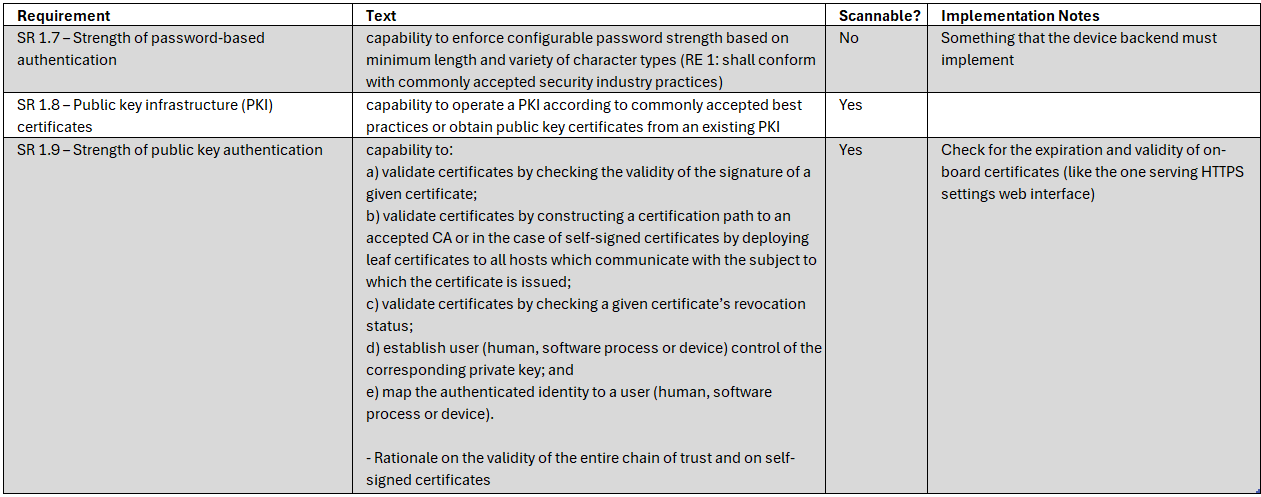
\includegraphics[width=1.0\textwidth]{chapters/04/assets/iec62443-findings-3_3}
  \caption{IEC 62443 \texttt{3-3} chosen requirements}
  \label{fig:iec62443-findings-3_3}
\end{figure}

\begin{figure}[t]
  \centering
  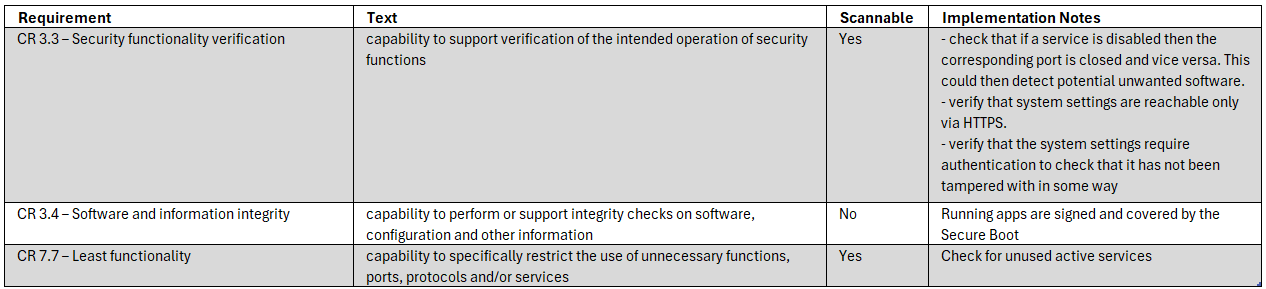
\includegraphics[width=1.0\textwidth]{chapters/04/assets/iec62443-findings-4_2}
  \caption{IEC 62443 \texttt{4-2} chosen requirements}
  \label{fig:iec62443-findings-4_2}
\end{figure}

To better explain our choices and motivations, we now take into account the \textit{SR 1.9 - Strength of public key authentication} requirement. The requirement states that there must be the capability to validate the validity of the used certificates by checking the signature, the expiration date, and the revocation status. We believe that this is a check that we should implement in the scanning tool because the user can fix the issue by itself by renewing the certificate, or by changing the certificate authority related to it if needed. The implementation of the check could be done by retrieving the certificate from the device and then checking the signature, the expiration date, and the revocation status. If the certificate is self-signed, the tool could suggest the user to change it with a certificate signed by a trusted certificate authority.

Instead, we now consider the \textit{SR 1.7 - Strength of password-based authentication}. The requirement states that the password must have a minimum length and a variety of character types. We put this assertion in a limbo, because if the user can set a password not respecting the requirement, the tool, which is a read-only intermediate between the user and the backend, cannot enforce the requirement. Then, the issue should be solved by the R\&D team, which should implement a password policy on the backend, and the user should be forced to change the password at the next login.

With this approach, we have identified the checks that the scanning tool should cover for sure from the standard, and we have included them in the backlog of the project.

\section{Agile method}

The \textit{Agile methodology} is a project management philosophy that involves breaking the project into phases and emphasizes continuous collaboration and improvement. Teams follow a cycle of planning, executing, and evaluating. Teams choose agile so they can respond to changes in the marketplace or feedback from customers quickly without derailing a year's worth of plans. The publication of the Agile Manifesto\footnote{\url{https://agilemanifesto.org}} in 2001 marks the birth of agile as a methodology. Since then, many agile frameworks have emerged such as scrum, kanban or lean. Each embodies the core principles of frequent iteration, continuous learning, and high quality in its own way.~\cite{agile-methodology} \\
We are now going to explain the Scrum framework, used by the company.

\subsection{Scrum}

Scrum is an agile project management framework, which is different from Agile, a philosophy.\\
The definition of scrum is based on empiricism and lean thinking. Empiricism says that knowledge comes from experience and that decisions are made based on what is observed. Lean thinking reduces waste and focuses on essentials. The scrum framework is heuristic; it is based on continuous learning and adjustment to fluctuating factors by acknowledging that the team does not know everything at the start of a project and it will evolve through experience. Scrum is structured to help teams to naturally adapt to changing conditions and user requirements, with re-prioritization built into the process and short release cycles so your team can constantly learn and improve.~\cite{scrum}

Scrum artefacts help to define the product, what work has to be done to create it and who has to do it. An \textit{epic} is a large body of work that can be broken down into smaller tasks. Each of these tasks is called \textit{story}, and it is a short requirement written from the perspective of an end user. The story is linked to a person in the team that has to carry it out.

The two main artefacts boards are the \textit{product backlog} and the \textit{sprint backlog}. \\
The former is a list of all the tasks that need to be done; it is a dynamic list of features, requirements, improvements, fixes and epics, ordered by their priority. Essentially, it is a \textit{"To Do"} list.\\
The latter is a list of items selected for the current sprint cycle; the sprint cycle is a fixed period of time, usually up to four weeks. Before each sprint, the team selects items from the product backlog to work on. Epics are broken down into stories, and stories are moved from the product backlog to the sprint backlog.~\cite{scrum-epic-stories}

\begin{figure}[t]
  \centering
  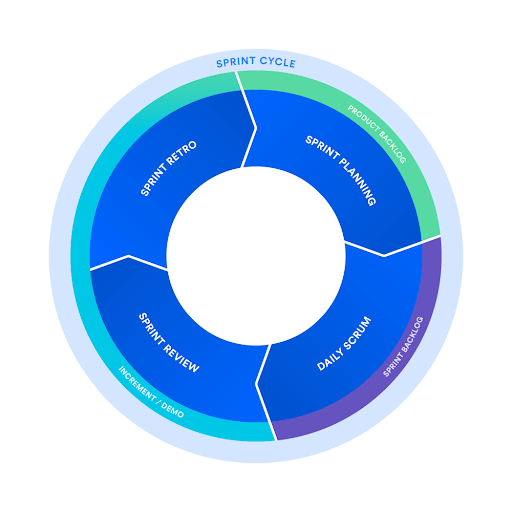
\includegraphics[width=0.8\textwidth]{chapters/04/assets/scrum}
  \caption{Scrum sprint cycle. Taken from \texttt{atlassian.com}}
  \label{fig:scrum-sprint-cycle}
\end{figure}

As visible in~\cref{fig:scrum-sprint-cycle}, Scrum is split in four principal phases:
\begin{itemize}
  \item The \textbf{sprint planning} is the initial phase of a sprint, the actual time period when the scrum team works; the team meets and decides what to do in the sprint by placing the tasks from the product backlog to the sprint backlog;
  \item The \textbf{daily scrum} is a quotidian meeting where the team members synchronize with each other. It is usually taken stand-up, as a way to not waste time and to keep the meeting short;
  \item The \textbf{sprint review} and \textbf{sprint retrospective} are the meetings at the end of the sprint where the team shows what they have done and demonstrates the work to the stakeholders and receive feedback;
\end{itemize}

The company takes advantage of the Scrum framework to manage the development of the cloud software, via the \textit{Jira} suite\footnote{\url{https://www.atlassian.com/software/jira}}, a proprietary project management tool developed by Atlassian. The tool is used to manage the product and the sprint backlog, the epics and the stories, and to track the progress of the team.

% TODO: Descrivere board di Jira, colonne, priorità

Given that we were part of the office team, together with the business tutor we created a new Epic for the scanning tool and we filled it with the stories that we thought were needed to develop the tool. In this specific case, the sprint period was two months because of the internship duration. At the end of the sprint, the product backlog contained some pending stories, because of the limited time and the ongoing updating of the priorities. The daily scrum was achieved by a quotidian quick meeting with the business tutor, where we keep him updated on the progress of the stories. Of course, new stories were added to the backlog, and some of them were de-prioritized.

\section{\textit{Go} programming language}

\textit{Go} is an open-source programming language supported by Google, designed for building simple, reliable, and efficient software. It is statically typed, compiled, and syntactically similar to C, with the added benefits of built-in concurrency management, garbage collection, memory safety, and a robust standard library plus packages. Go is widely used in cloud computing, web development, and systems programming due to its simplicity, performance, and scalability.~\cite{go-lang-site}~\cite{go-lang-wikipedia}\\
Go was released in 2007 by Google, and at the time of writing it is at version \texttt{1.22}.

\begin{figure}[h]
  \centering
  
\includegraphics[width=0.9\textwidth]{chapters/04/assets/golang}
  \caption{Go logo and mascot. Taken from \texttt{nixsolutions.com}}
  \label{fig:go-logo-mascot}
\end{figure}

Go's standard library provides comprehensive support for networking, encryption, and concurrency. The built-in packages for HTTP, TLS, and JSON processing simplify the implementation of RESTful APIs, secure communication channels, and data serialization/deserialization, respectively. If additional functionalities are required, the language supports third-party packages through the Go module system; in order to download a custom package, the developer simply references it in the code via the link to the repository, and the Go compiler will automatically download and install it.

Go also offers a robust testing framework to write unit tests and benchmarks to ensure the reliability and performance of their code. The testing framework is integrated into the language and provides a simple and efficient way to write tests for functions and methods. The testing framework also supports the generation of code coverage reports to identify untested code paths and improve the overall test coverage. Furthermore, Go's testing framework supports the use of table-driven tests, which allow the developer to define test cases in a structured format and iterate over them to execute the tests and also it supports fuzzing, a technique used to discover vulnerabilities in software by providing random or invalid inputs to the program.

Another point in favor is the efficiency of the language. Go is compiled into machine code, which makes it faster than interpreted languages like Python. The language's garbage collection mechanism automatically manages memory allocation and deallocation, reducing the risk of memory leaks and improving the overall performance of the application. The language is more than a full order of magnitude faster than Python, with a smaller memory footprint and faster execution times.~\cite{go-lang-performance}

One of the main reasons for choosing Go for the internship project is its versatility in building executable binaries for multiple platforms, including Windows, macOS, and Linux. Go's cross-compilation capabilities allow the developers to build binaries for different operating systems and architectures from a single codebase, simplifying the deployment process and ensuring compatibility across various platforms. Given that industrial devices run on different architectures and operating systems, the ability to build cross-platform binaries is essential. The language natively supports the binaries compilation for over 50 combinations of operating systems and architectures~\cite{go-lang-compilation-combo}; given that the majority of the company's devices run either on \texttt{Arm 32bit} or \texttt{Arm 64bit} or \texttt{x86 64bit} architectures, the Go compiler can generate the executables for these architectures with no further configuration needed.


% TODO: libraries

